\documentclass[a4j,11pt]{jarticle}
\usepackage{fancyheadings}
\usepackage{here}
\usepackage[dvipdfmx]{graphicx}
\renewcommand{\thepage}{\small -- \arabic{page} --}
%\headrulewidth=0pt
\rhead{}
\lhead{}
\textheight 234mm
%
\usepackage{amsmath,amssymb}
\usepackage{bm}
\usepackage{ascmac}
\usepackage{color}
\usepackage{listings,jvlisting}
\usepackage{enumerate}
\usepackage{url}
\newcommand{\thisyear}{1}
\pagestyle{fancy}
\lhead{{\number\year}年度 信号処理特論1}
\title{{\number\year}年度 信号処理特論1}
\date{\number\year 年\number\month 月\number\day 日}
\author{36414067  飯田 諒 \\ メディア情報プログラム\\徳田・南角・橋本研究室}
%
%
\lstset{
    language=Python,
    commentstyle=\color{gray}\ttfamily,
    basicstyle={\ttfamily},
    identifierstyle={\small},
    commentstyle={\smallitshape},
    keywordstyle={\small\bfseries},
    ndkeywordstyle={\small},
    stringstyle={\small\ttfamily},
    frame={tb},
    breaklines=true,
    columns=[l]{fullflexible},
    numbers=left,
    xrightmargin=0zw,
    xleftmargin=3zw,
    numberstyle={\scriptsize},
    stepnumber=1,
    numbersep=1zw,
    lineskip=-0.5ex
}
\begin{document}
    \maketitle
    \thispagestyle{empty}
    \clearpage
    
    \begin{itemize}
        \item 使用した音:自分自身の声
        \item 使用したソフト:WaveSufer
        \item 使用した機材:自身の計算機
        \item 使用したOS:Windows
        \item プログラミング言語:Python
    \end{itemize}
    課題のソースコードは資料の最後尾にまとめて載せる。
    \section{課題1}
    \subsection{内容}
    ヘッダには、ファイルの形式、ファイルサイズ等の、ファイル自体の情報を示すものが書かれていた。
    具体的には先端から順に以下のとおりである。\\
    52 49 46 46 : "RIFF"\\
    24 fa 00 00 : ファイルサイズ\\
    57 41 56 45 : "WAVE"\\
    66 6d 74 20 : "fmt"\\
    10 00 00 00: fmtチャンクのサイズ\\
    01 00: オーディオフォーマット\\
    01 00: チャンネル数\\
    80 3e 00 00: サンプリングレート\\
    00 7d 00 00: バイトレート\\
    02 00: ブロックアライン\\
    10 00: ビット数\\
    64 61 74 61: "data"\\
    00 fa 00 00 ... : データの中身\\
    \\
    データの中身に置ける10番目の値は、00 00であったため、0である。
    \subsection{ソースコード}
    
    \section{課題2}
    図\ref{fig:2}に示すとおりである。
    \begin{figure}[tb]
        \centering
        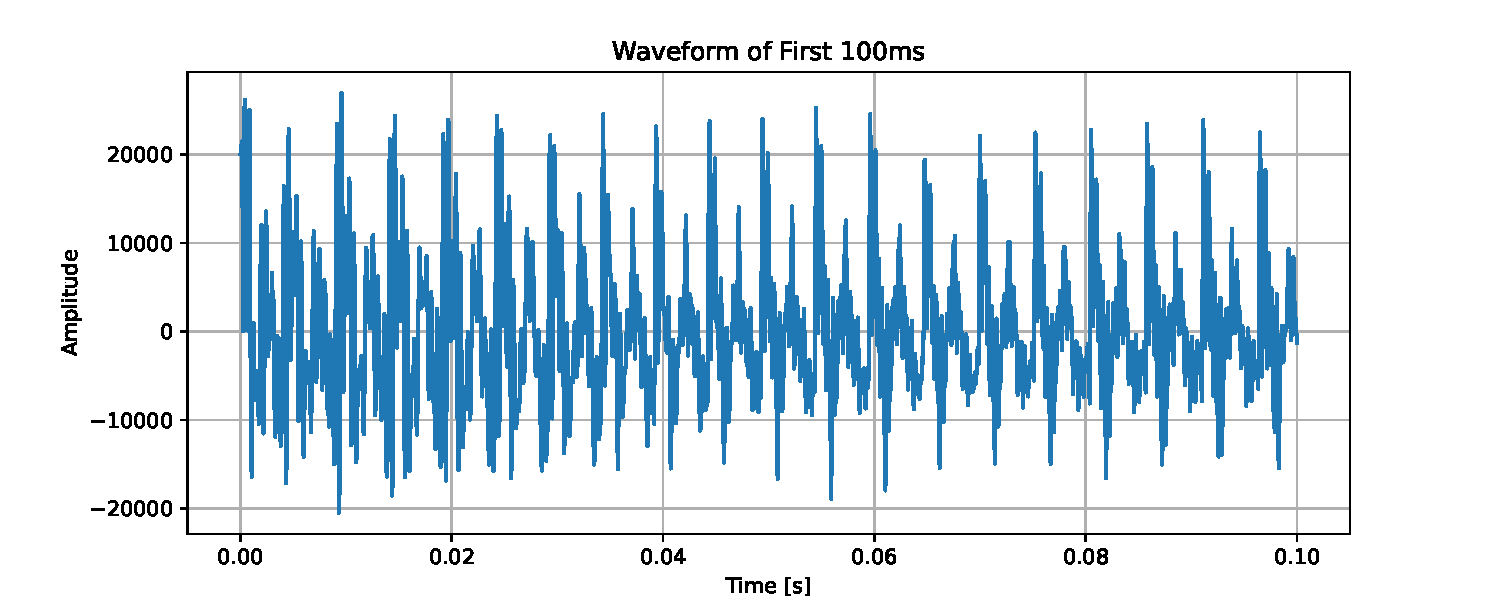
\includegraphics[width=0.8\hsize]{../../figure/dataplot_arayurugennzituwo.pdf}
        \caption{先頭100msecのプロット}
        \label{fig:2}
    \end{figure}
    \section{課題3}
    \subsection{方法}
    正規化は、音声の数値データの最大値と、-3dBFSの最大値である23170.47との比を取る。その後、音声データの数値すべてに対して算出した比を掛け算し、int型にする。\\
    量子ビット数の変更は、データに対してそれぞれ、$2^{8},2^{12}$で割り、int型にして、$2^{8},2^{12}$を掛けた。
    \subsection{結果}
    図\ref{fig:3-1}、図\ref{fig:3-2}に示すとおりである。
    \begin{figure}[tb]
        \centering
        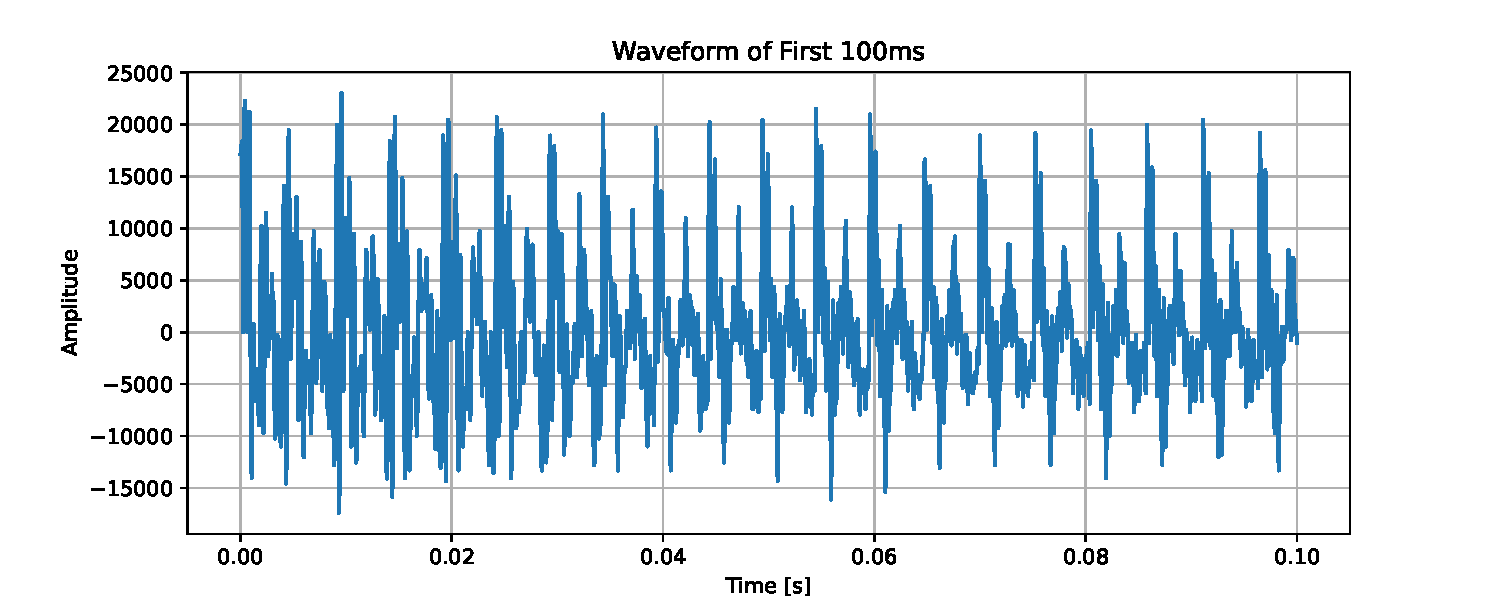
\includegraphics[width=0.8\hsize]{../../figure/dataplot_8bit_arayurugennzituwo.pdf}
        \caption{量子ビット数を$\frac 1 2$へ}
        \label{fig:3-1}
    \end{figure}
    \begin{figure}[tb]
        \centering
        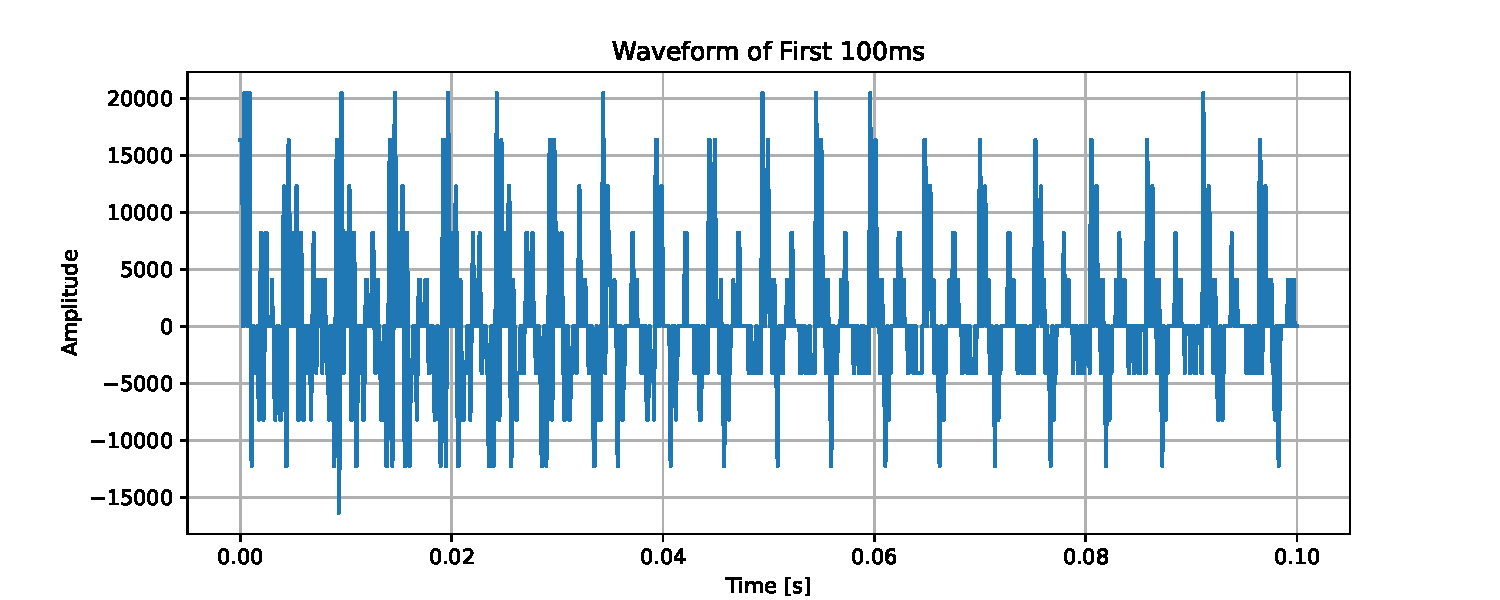
\includegraphics[width=0.8\hsize]{../../figure/dataplot_4bit_arayurugennzituwo.pdf}
        \caption{量子ビット数を$\frac 1 4$へ}
        \label{fig:3-2}
    \end{figure}
    \section{課題4}
    量子ビット数を$\frac 1 2$にしたものは、声の音質の劣化は感じ取ることが出来なかったが、声を出すたびに、「ザッ」というノイズが少し乗っているように聞こえた。\\
    量子ビット数を$\frac 1 4$にしたものは、明らかに音質の劣化が見られ、ノイズが組み合わさってできたような声、ブツブツとした声に感じた。\\
    \section{課題5}
    図\ref{fig:5-1}、図\ref{fig:5-2}に示すとおりである。
    \begin{figure}[tb]
        \centering
        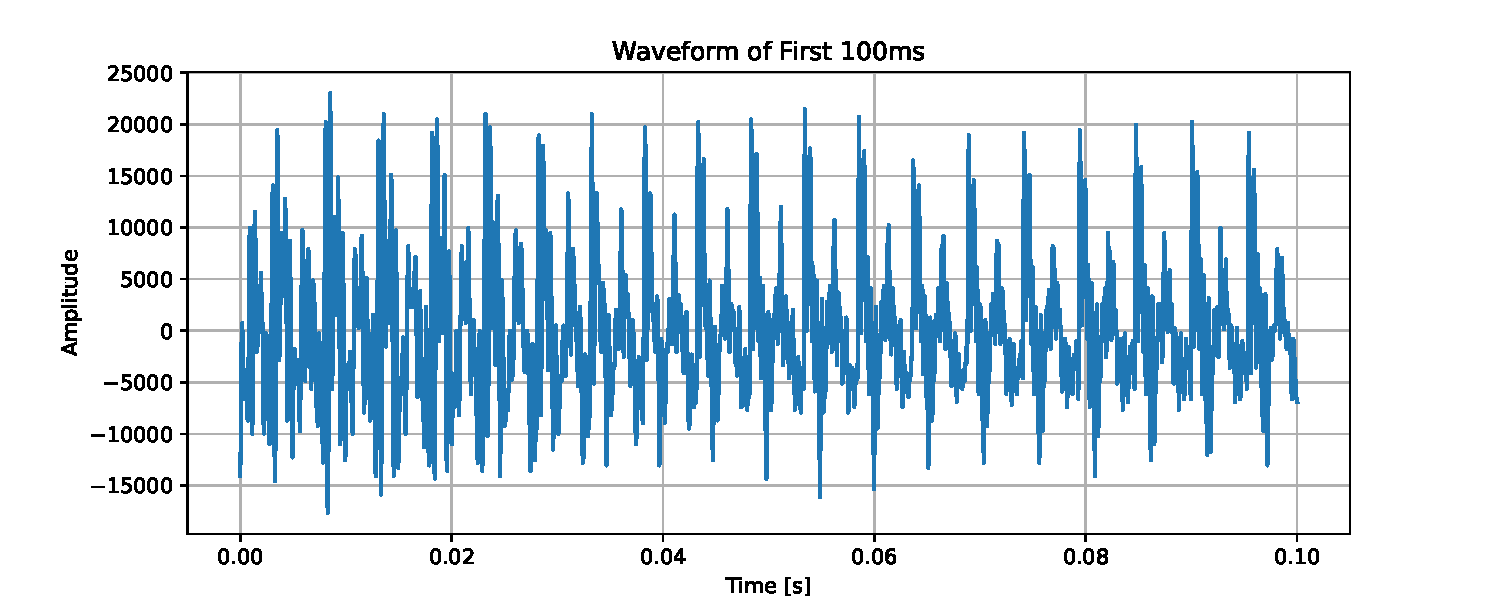
\includegraphics[width=0.8\hsize]{../../figure/dataplot_8bit_reconst_linear_interpolation_arayurugennzituwo.pdf}
        \caption{量子ビット数を$\frac 1 2$に変換後、線形補間}
        \label{fig:5-1}
    \end{figure}
    \begin{figure}[tb]
        \centering
        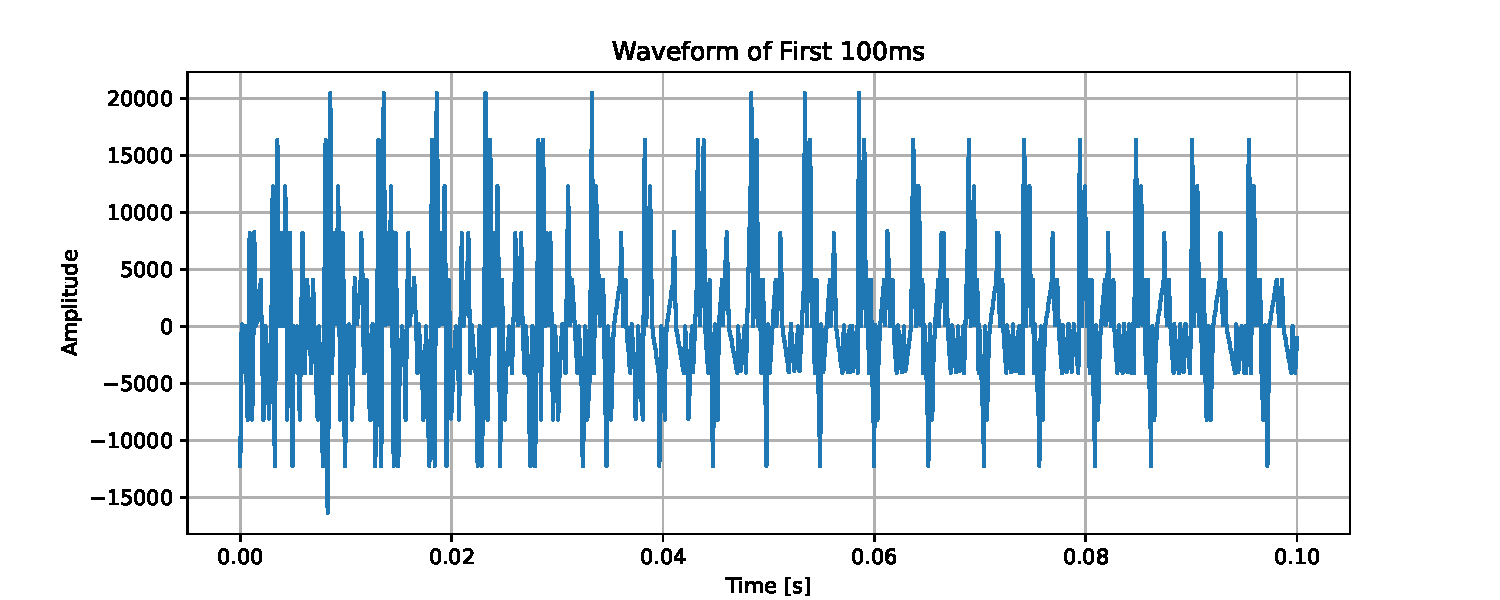
\includegraphics[width=0.8\hsize]{../../figure/dataplot_4bit_reconst_linear_interpolation_arayurugennzituwo.pdf}
        \caption{量子ビット数を$\frac 1 4$に変換後、線形補間}
        \label{fig:5-2}
    \end{figure}
    線形補間のようなことをした。例を挙げると、-8, 2, 2, 2, 2, 2, 2, 8, ...という音声データが存在するとき、
    連続する値である2に注目して、最初に現れた2と、連続した2の次に現れる8を滑らかにつなぐように線形で補間をし、
    -8, 2, 3, 4, 5, 6, 7, 8, ...となるようにした。\\
    量子ビット数を$\frac 1 2$にしたものは、「ザッ」といったノイズの音自体が低くなり、目立たなくなったように感じた。\\
    量子ビット数を$\frac 1 4$にしたものは、音質の劣化は改善できなかったが、高いノイズの音が、低くなっているように感じた。\\
    線形補間を行った考察として、急激な値の変化に対応する高周波成分を、線形補間を行うことによって緩やかな値の変化に変換したことによって
    低周波成分に変わったと考える。
    
    \section{ソースコードの主要部}
    \subsection{課題1}
    \begin{lstlisting}[language=Python, caption=binary.py]
filename= "arayurugennzituwo"
with open('{}.wav'.format(filename), 'rb') as f:
    data = f.read()

mystr = ""
i = 0
while i < len(data)-1 :
datai = int(data[i])
if i <= 40 :
    if  (65 <= datai <= 90 or 97 <= datai <= 122) :
        mystr = mystr + " " + chr(datai)
    else :
        mystr = mystr + " " + str(datai)
    i += 1
else :
    datai *=256
    datai += int(data[i+1])
    if datai > 32767 :
        datai -= 65536
    mystr = mystr + " " + str(datai)
    i += 2

with open('{}.txt'.format(filename), 'w') as output_file:
output_file.write(mystr)
    \end{lstlisting}
    \subsection{課題2}
    \begin{lstlisting}[language=Python, caption=dataplot.py]
sampling_rate = 16000
max_time = 0.1
fleng = int(max_time*sampling_rate)
time = np.linspace(0,max_time,fleng)
fdata_short = fdata[:fleng].copy()
if __name__ == "__main__" :
    plt.figure(figsize=(10,4))
    plt.plot(time,fdata_short)
    plt.title("Waveform of First 100ms")
    plt.xlabel("Time [s]")
    plt.ylabel("Amplitude")
    plt.grid()
    plt.savefig("../figure/dataplot_{}.pdf".format(fname))
    \end{lstlisting}
    \subsection{課題3}
    \begin{lstlisting}[language = Python, caption = bitdown.py]
downbit = 12

def normalization(data) :
    full_scale = 32767
    minus_3dbfs = full_scale / np.sqrt(2)

    normal_scale = minus_3dbfs/data.max()
    norm_data = (data*normal_scale).astype(int)
    return norm_data

def down(data, downbit) :
    size = 1 << downbit
    down_data = (data/size).astype(int)
    down_data = down_data*size

    return down_data
        
    \end{lstlisting}
    \subsection{課題4}
    \begin{lstlisting}[language=Python, caption=reconst.py]
import scipy.io.wavfile as wavfile

downbit = 8

if __name__ == "__main__" :
    input_wav_file = fpath + ".wav"
    output_wav_file = '{}bit_reconst_{}.wav'.format(16-downbit,fname)
    sampling_rate, data = wavfile.read(input_wav_file)

    norm_data = normalization(data)
    down_data = down(norm_data,downbit).astype(np.int16)

    wavfile.write(output_wav_file, sampling_rate, down_data)
        
    \end{lstlisting}
    \subsection{課題5}
    \begin{lstlisting}[language=Python, caption=liear\_interpolation.py]
li = 0
for ri in range(len(down_data)) :
    if down_data[li] != down_data[ri] :
        l = down_data[li]
        r = down_data[ri]
        leng = ri - li
        for j in range(leng) :
            down_data[li+j] = int(l + (r - l) * j/leng)
        li = ri
    \end{lstlisting}
    \end{document}